
\begin{figure}[H]
  {
    \setlength{\tabcolsep}{3.0pt}
    \setlength\cmidrulewidth{\heavyrulewidth} % Make cmidrule = 
    \begin{adjustbox}{height=2cm,center}
      \footnotesize
      \begin{tabular}{ll}

        \makecell[l]{
\icode{.BYTE \$FD,\$03}\\
\icode{.BYTE \$FF,\$FF}
} & \makecell[l]{

\includegraphics[width=1.3cm]{src/colorspace_patterns/pixels/pixel_pattern11_2.png}%

\includegraphics[width=1.3cm]{src/colorspace_patterns/pixels/pixel_pattern11_3.png}%
} \\
        \midrule

        \makecell[l]{
\icode{.BYTE \$FA,\$06}\\
\icode{.BYTE \$01,\$01}
} & \makecell[l]{

\includegraphics[width=1.3cm]{src/colorspace_patterns/pixels/pixel_pattern11_4.png}%
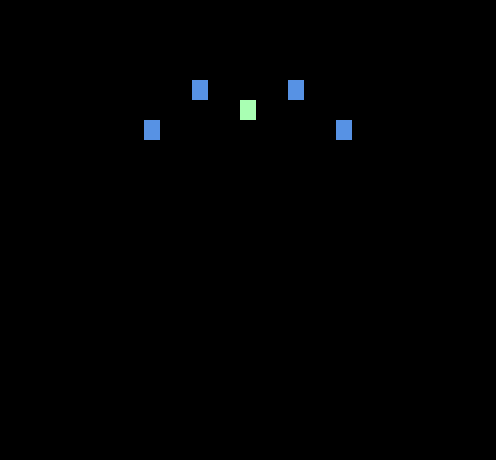
\includegraphics[width=1.3cm]{src/colorspace_patterns/pixels/pixel_pattern11_5.png}%
} \\
        \midrule

        \makecell[l]{
\icode{.BYTE \$F8,\$07}\\
\icode{.BYTE \$FC,\$FC}
} & \makecell[l]{
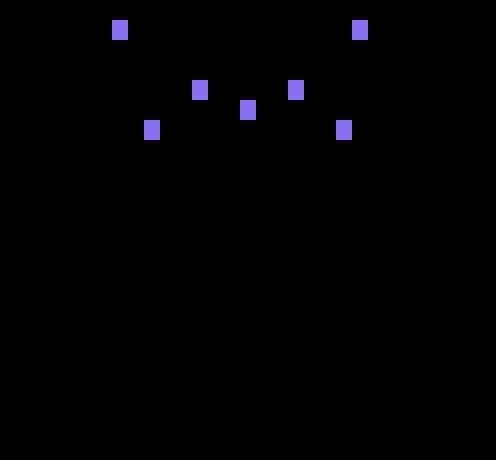
\includegraphics[width=1.3cm]{src/colorspace_patterns/pixels/pixel_pattern11_6.png}%
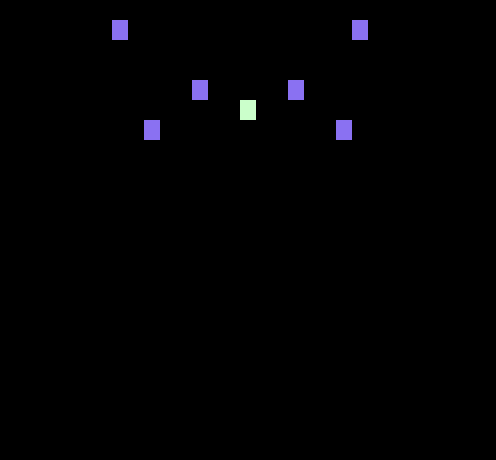
\includegraphics[width=1.3cm]{src/colorspace_patterns/pixels/pixel_pattern11_7.png}%
} \\
        \midrule

        \makecell[l]{
\icode{.BYTE \$F4,\$0C}\\
\icode{.BYTE \$02,\$02}
} & \makecell[l]{
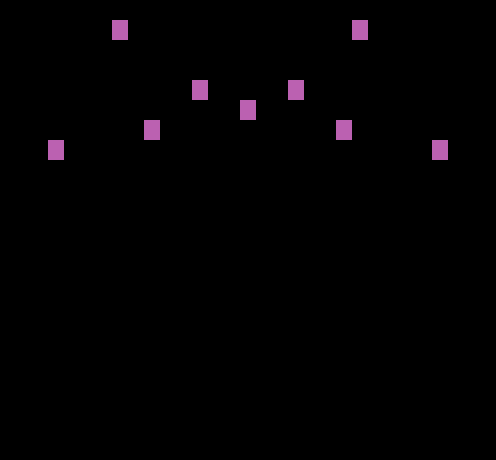
\includegraphics[width=1.3cm]{src/colorspace_patterns/pixels/pixel_pattern11_8.png}%
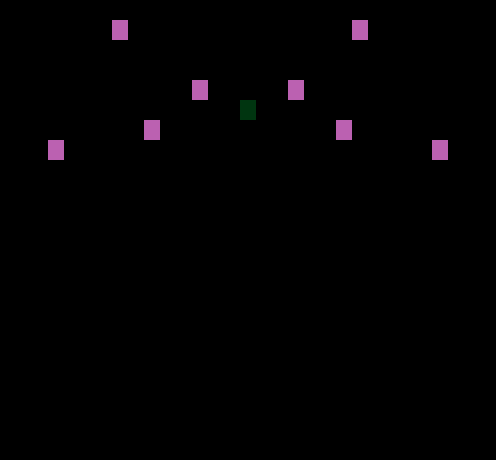
\includegraphics[width=1.3cm]{src/colorspace_patterns/pixels/pixel_pattern11_9.png}%
} \\
        \midrule

        \makecell[l]{
\icode{.BYTE \$F3,\$F1,\$0D,\$0F}\\
\icode{.BYTE \$04,\$04,\$04,\$04}
} & \makecell[l]{
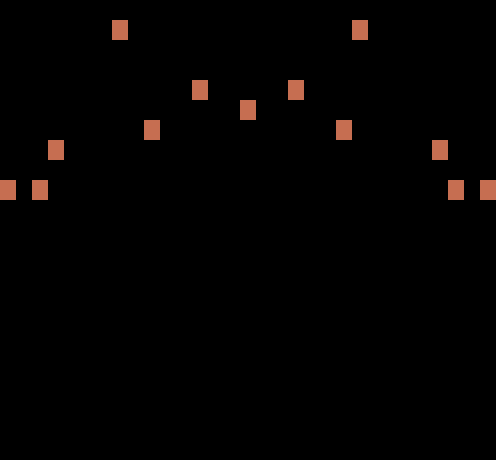
\includegraphics[width=1.3cm]{src/colorspace_patterns/pixels/pixel_pattern11_10.png}%
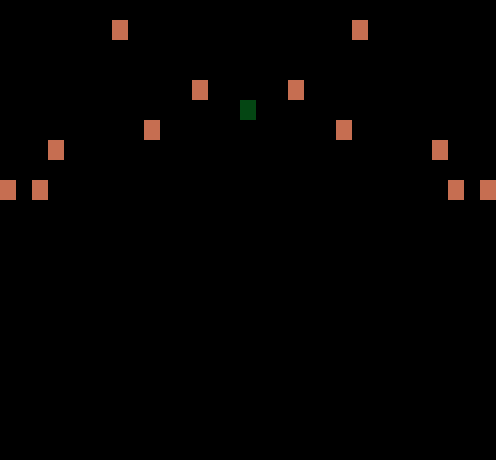
\includegraphics[width=1.3cm]{src/colorspace_patterns/pixels/pixel_pattern11_11.png}%
} \\
        \midrule

        \makecell[l]{
\icode{.BYTE \$00,\$00,\$00}\\
\icode{.BYTE \$FB,\$0A,\$11}
} & \makecell[l]{
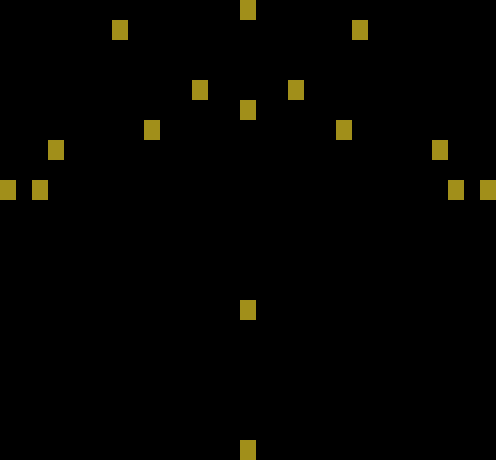
\includegraphics[width=1.3cm]{src/colorspace_patterns/pixels/pixel_pattern11_12.png}%
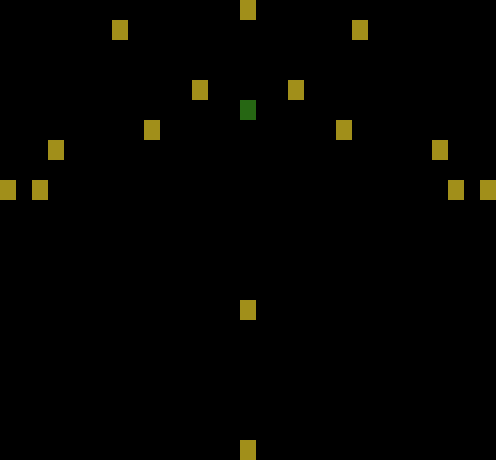
\includegraphics[width=1.3cm]{src/colorspace_patterns/pixels/pixel_pattern11_13.png}%
} \\
        \midrule

          \end{tabular}
        \end{adjustbox}
      }
    \end{figure}
    
